\documentclass[twoside]{book}

% Packages required by doxygen
\usepackage{calc}
\usepackage{doxygen}
\usepackage{graphicx}
\usepackage[utf8]{inputenc}
\usepackage{makeidx}
\usepackage{multicol}
\usepackage{multirow}
\usepackage{textcomp}
\usepackage[table]{xcolor}

% Font selection
\usepackage[T1]{fontenc}
\usepackage{mathptmx}
\usepackage[scaled=.90]{helvet}
\usepackage{courier}
\usepackage{amssymb}
\usepackage{sectsty}
\renewcommand{\familydefault}{\sfdefault}
\allsectionsfont{%
  \fontseries{bc}\selectfont%
  \color{darkgray}%
}
\renewcommand{\DoxyLabelFont}{%
  \fontseries{bc}\selectfont%
  \color{darkgray}%
}

% Page & text layout
\usepackage{geometry}
\geometry{%
  a4paper,%
  top=2.5cm,%
  bottom=2.5cm,%
  left=2.5cm,%
  right=2.5cm%
}
\tolerance=750
\hfuzz=15pt
\hbadness=750
\setlength{\emergencystretch}{15pt}
\setlength{\parindent}{0cm}
\setlength{\parskip}{0.2cm}
\makeatletter
\renewcommand{\paragraph}{%
  \@startsection{paragraph}{4}{0ex}{-1.0ex}{1.0ex}{%
    \normalfont\normalsize\bfseries\SS@parafont%
  }%
}
\renewcommand{\subparagraph}{%
  \@startsection{subparagraph}{5}{0ex}{-1.0ex}{1.0ex}{%
    \normalfont\normalsize\bfseries\SS@subparafont%
  }%
}
\makeatother

% Headers & footers
\usepackage{fancyhdr}
\pagestyle{fancyplain}
\fancyhead[LE]{\fancyplain{}{\bfseries\thepage}}
\fancyhead[CE]{\fancyplain{}{}}
\fancyhead[RE]{\fancyplain{}{\bfseries\leftmark}}
\fancyhead[LO]{\fancyplain{}{\bfseries\rightmark}}
\fancyhead[CO]{\fancyplain{}{}}
\fancyhead[RO]{\fancyplain{}{\bfseries\thepage}}
\fancyfoot[LE]{\fancyplain{}{}}
\fancyfoot[CE]{\fancyplain{}{}}
\fancyfoot[RE]{\fancyplain{}{\bfseries\scriptsize Generated on Sun Apr 20 2014 22\-:09\-:37 for Particle\-Editor by Doxygen }}
\fancyfoot[LO]{\fancyplain{}{\bfseries\scriptsize Generated on Sun Apr 20 2014 22\-:09\-:37 for Particle\-Editor by Doxygen }}
\fancyfoot[CO]{\fancyplain{}{}}
\fancyfoot[RO]{\fancyplain{}{}}
\renewcommand{\footrulewidth}{0.4pt}
\renewcommand{\chaptermark}[1]{%
  \markboth{#1}{}%
}
\renewcommand{\sectionmark}[1]{%
  \markright{\thesection\ #1}%
}

% Indices & bibliography
\usepackage{natbib}
\usepackage[titles]{tocloft}
\setcounter{tocdepth}{3}
\setcounter{secnumdepth}{5}
\makeindex

% Hyperlinks (required, but should be loaded last)
\usepackage{ifpdf}
\ifpdf
  \usepackage[pdftex,pagebackref=true]{hyperref}
\else
  \usepackage[ps2pdf,pagebackref=true]{hyperref}
\fi
\hypersetup{%
  colorlinks=true,%
  linkcolor=blue,%
  citecolor=blue,%
  unicode%
}

% Custom commands
\newcommand{\clearemptydoublepage}{%
  \newpage{\pagestyle{empty}\cleardoublepage}%
}


%===== C O N T E N T S =====

\begin{document}

% Titlepage & ToC
\hypersetup{pageanchor=false}
\pagenumbering{roman}
\begin{titlepage}
\vspace*{7cm}
\begin{center}%
{\Large Particle\-Editor }\\
\vspace*{1cm}
{\large Generated by Doxygen 1.8.6}\\
\vspace*{0.5cm}
{\small Sun Apr 20 2014 22:09:37}\\
\end{center}
\end{titlepage}
\clearemptydoublepage
\tableofcontents
\clearemptydoublepage
\pagenumbering{arabic}
\hypersetup{pageanchor=true}

%--- Begin generated contents ---
\chapter{Hierarchical Index}
\section{Class Hierarchy}
This inheritance list is sorted roughly, but not completely, alphabetically\-:\begin{DoxyCompactList}
\item \contentsline{section}{Particle\-Model}{\pageref{class_particle_model}}{}
\item Q\-Main\-Window\begin{DoxyCompactList}
\item \contentsline{section}{Main\-Window}{\pageref{class_main_window}}{}
\end{DoxyCompactList}
\item \contentsline{section}{Util}{\pageref{class_util}}{}
\item \contentsline{section}{X\-M\-L}{\pageref{class_x_m_l}}{}
\end{DoxyCompactList}

\chapter{Class Index}
\section{Class List}
Here are the classes, structs, unions and interfaces with brief descriptions\-:\begin{DoxyCompactList}
\item\contentsline{section}{\hyperlink{class_main_window}{Main\-Window} }{\pageref{class_main_window}}{}
\item\contentsline{section}{\hyperlink{class_particle_model}{Particle\-Model} }{\pageref{class_particle_model}}{}
\item\contentsline{section}{\hyperlink{class_util}{Util} }{\pageref{class_util}}{}
\item\contentsline{section}{\hyperlink{class_x_m_l}{X\-M\-L} }{\pageref{class_x_m_l}}{}
\end{DoxyCompactList}

\chapter{Class Documentation}
\hypertarget{class_main_window}{\section{Main\-Window Class Reference}
\label{class_main_window}\index{Main\-Window@{Main\-Window}}
}
Inheritance diagram for Main\-Window\-:\begin{figure}[H]
\begin{center}
\leavevmode
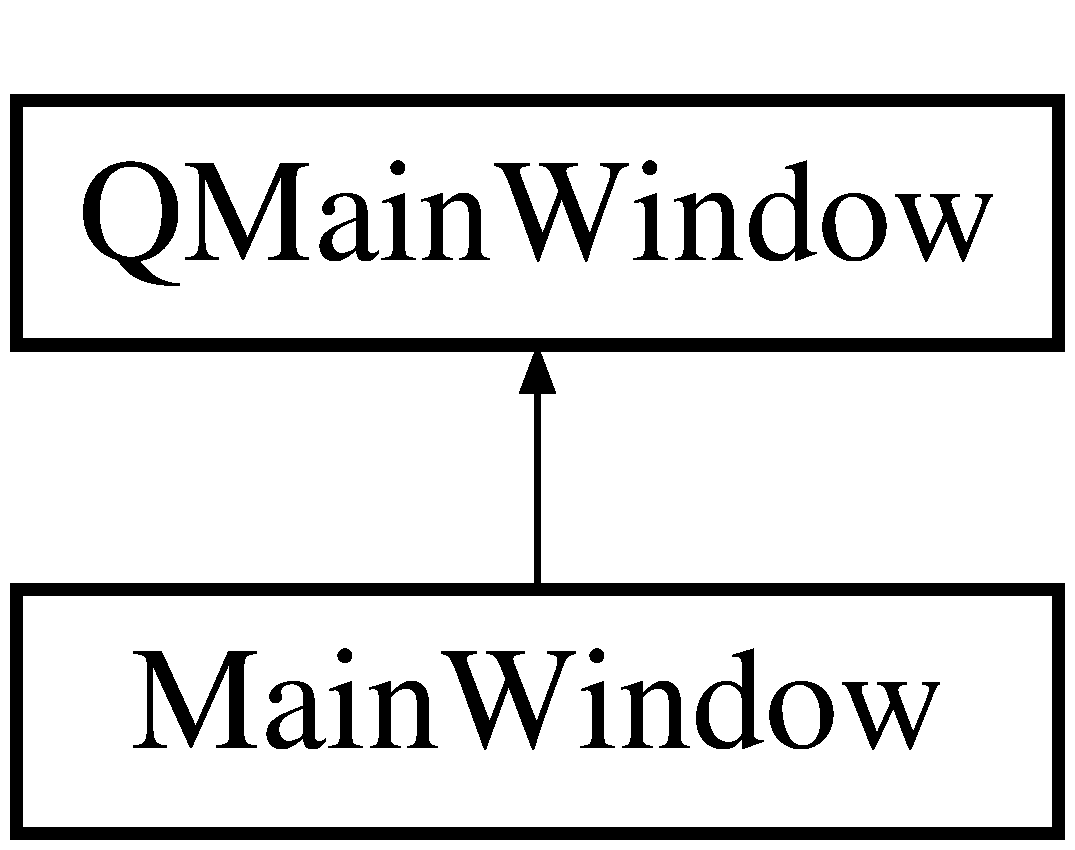
\includegraphics[height=2.000000cm]{class_main_window}
\end{center}
\end{figure}
\subsection*{Public Member Functions}
\begin{DoxyCompactItemize}
\item 
\hypertarget{class_main_window_a8b244be8b7b7db1b08de2a2acb9409db}{{\bfseries Main\-Window} (Q\-Widget $\ast$parent=0)}\label{class_main_window_a8b244be8b7b7db1b08de2a2acb9409db}

\item 
\hypertarget{class_main_window_ab0f6b9144b6b8188bcbfd4a874cf2cab}{void {\bfseries set\-Particle\-Model} (\hyperlink{class_particle_model}{Particle\-Model} $\ast$model)}\label{class_main_window_ab0f6b9144b6b8188bcbfd4a874cf2cab}

\end{DoxyCompactItemize}


The documentation for this class was generated from the following files\-:\begin{DoxyCompactItemize}
\item 
mainwindow.\-h\item 
mainwindow.\-cpp\end{DoxyCompactItemize}

\hypertarget{class_particle_model}{\section{Particle\-Model Class Reference}
\label{class_particle_model}\index{Particle\-Model@{Particle\-Model}}
}
\subsection*{Public Types}
\begin{DoxyCompactItemize}
\item 
enum \hyperlink{class_particle_model_a20dbdb2c6762bb19a57cb1553f73051f}{Emitter\-Types} \{ \\*
{\bfseries N\-O\-N\-E} = 0, 
{\bfseries B\-O\-X} = 1, 
{\bfseries P\-O\-I\-N\-T} = 2, 
{\bfseries A\-N\-I\-M\-A\-T\-E\-D\-\_\-\-M\-E\-S\-H} = 3, 
\\*
{\bfseries C\-Y\-L\-I\-N\-D\-E\-R} = 4, 
{\bfseries M\-E\-S\-H} = 5, 
{\bfseries R\-I\-N\-G} = 6, 
{\bfseries S\-P\-H\-E\-R\-E} = 7
 \}
\end{DoxyCompactItemize}
\subsection*{Public Member Functions}
\begin{DoxyCompactItemize}
\item 
\hyperlink{class_particle_model_a10f4ad88fb013be6f42d86012490d0b6}{Particle\-Model} ()
\item 
void \hyperlink{class_particle_model_a0632fbf8ac2805c1235fa28f7ee42a4b}{set\-Emitter\-Type} (\hyperlink{class_particle_model_a20dbdb2c6762bb19a57cb1553f73051f}{Emitter\-Types} emitter\-Type)
\item 
\hypertarget{class_particle_model_a4c6fe1f0723ff83f087a26b1d0b758a0}{void {\bfseries set\-Aabbox} (core\-::aabbox3df aabbox)}\label{class_particle_model_a4c6fe1f0723ff83f087a26b1d0b758a0}

\item 
\hypertarget{class_particle_model_a2cfd58da58cea46b8ba4e7131a85379f}{void {\bfseries set\-Direction} (core\-::vector3df direction)}\label{class_particle_model_a2cfd58da58cea46b8ba4e7131a85379f}

\item 
\hypertarget{class_particle_model_acea094d5b21057e397b094e44dfa1c37}{void {\bfseries set\-Position} (core\-::vector3df position)}\label{class_particle_model_acea094d5b21057e397b094e44dfa1c37}

\item 
\hypertarget{class_particle_model_ab3420eaf505d35a6f96bb582c981b13f}{void {\bfseries set\-Center} (core\-::vector3df center)}\label{class_particle_model_ab3420eaf505d35a6f96bb582c981b13f}

\item 
\hypertarget{class_particle_model_abd2f6620ef31fc7e63e356830c0d6849}{void {\bfseries set\-Normal} (core\-::vector3df normal)}\label{class_particle_model_abd2f6620ef31fc7e63e356830c0d6849}

\item 
\hypertarget{class_particle_model_a7fb55c77d94011525ee27dfed38b4734}{void {\bfseries set\-Max\-Angle\-Degrees} (s32 max\-Angle\-Degrees)}\label{class_particle_model_a7fb55c77d94011525ee27dfed38b4734}

\item 
\hypertarget{class_particle_model_aaaf9ea758b3ad884d0885cf38265b7bb}{void {\bfseries set\-Mb\-Number} (s32 mb\-Number)}\label{class_particle_model_aaaf9ea758b3ad884d0885cf38265b7bb}

\item 
\hypertarget{class_particle_model_a9dc4570da03895afb9ab8094b8035991}{void {\bfseries set\-Life\-Time\-Max} (u32 life\-Time\-Max)}\label{class_particle_model_a9dc4570da03895afb9ab8094b8035991}

\item 
\hypertarget{class_particle_model_a3d94a2ab52b078b67d37b14cd2213bdf}{void {\bfseries set\-Life\-Time\-Min} (u32 life\-Time\-Min)}\label{class_particle_model_a3d94a2ab52b078b67d37b14cd2213bdf}

\item 
\hypertarget{class_particle_model_aa6ab281bda3309140247f0774d59f3f6}{void {\bfseries set\-Max\-P\-P\-S} (u32 max\-P\-P\-S)}\label{class_particle_model_aa6ab281bda3309140247f0774d59f3f6}

\item 
\hypertarget{class_particle_model_a3d67b143881897ea4df87f566bc26edc}{void {\bfseries set\-Min\-P\-P\-S} (u32 min\-P\-Ps)}\label{class_particle_model_a3d67b143881897ea4df87f566bc26edc}

\item 
\hypertarget{class_particle_model_abdb963e9e65cf735163c1c42622b4905}{void {\bfseries set\-Normal\-Direction\-Modifier} (f32 normal\-Direction\-Modifier)}\label{class_particle_model_abdb963e9e65cf735163c1c42622b4905}

\item 
\hypertarget{class_particle_model_a8a8b80fd5978788cb6b2cd8c0c625855}{void {\bfseries set\-Radius} (f32 radius)}\label{class_particle_model_a8a8b80fd5978788cb6b2cd8c0c625855}

\item 
\hypertarget{class_particle_model_aa9f354658c7b81ffe378a88bf42ad6fd}{void {\bfseries set\-Length\-Cylinder} (f32 length\-Cylinder)}\label{class_particle_model_aa9f354658c7b81ffe378a88bf42ad6fd}

\item 
\hypertarget{class_particle_model_adad7df1e4ec075ffb86d32ffea4b199f}{void {\bfseries set\-Ring\-Thickness} (f32 ring\-Thickness)}\label{class_particle_model_adad7df1e4ec075ffb86d32ffea4b199f}

\item 
\hypertarget{class_particle_model_ac44eeca675b5bd7b72974eec8386968d}{void {\bfseries set\-Path\-Name\-Texture} (core\-::stringc path\-Name\-Texture)}\label{class_particle_model_ac44eeca675b5bd7b72974eec8386968d}

\item 
\hypertarget{class_particle_model_adfe0b83b4c25c4e613e051422bdd1349}{void {\bfseries set\-Min\-Color} (video\-::\-S\-Color min\-Color)}\label{class_particle_model_adfe0b83b4c25c4e613e051422bdd1349}

\item 
\hypertarget{class_particle_model_a4410a41c677b700eb9358916414e3293}{void {\bfseries set\-Max\-Color} (video\-::\-S\-Color max\-Color)}\label{class_particle_model_a4410a41c677b700eb9358916414e3293}

\item 
\hypertarget{class_particle_model_af8b287d8b304e9863399d14273810567}{void {\bfseries set\-Min\-Start\-Size} (core\-::dimension2df min\-Start\-Size)}\label{class_particle_model_af8b287d8b304e9863399d14273810567}

\item 
\hypertarget{class_particle_model_a5ce6ed84f6208430e09b690b829f4527}{void {\bfseries set\-Max\-Start\-Size} (core\-::dimension2df max\-Start\-Size)}\label{class_particle_model_a5ce6ed84f6208430e09b690b829f4527}

\item 
\hypertarget{class_particle_model_a9bd71de9e4797e2953506acebb075c17}{void {\bfseries set\-Use\-Normal\-Direction} (bool use\-Normal\-Direction)}\label{class_particle_model_a9bd71de9e4797e2953506acebb075c17}

\item 
\hypertarget{class_particle_model_ac293853e0f24a2381de32e22bdf4fbdb}{void {\bfseries set\-Every\-Mesh\-Vertex} (bool ever\-Mesh\-Vertex)}\label{class_particle_model_ac293853e0f24a2381de32e22bdf4fbdb}

\item 
\hypertarget{class_particle_model_ac26bcb202c3e649cd57af8423cc83ffd}{void {\bfseries set\-Out\-Line\-Only} (bool outline\-Only)}\label{class_particle_model_ac26bcb202c3e649cd57af8423cc83ffd}

\item 
\hyperlink{class_particle_model_a20dbdb2c6762bb19a57cb1553f73051f}{Emitter\-Types} \hyperlink{class_particle_model_a9d604becd6847bb1668d3bce13c230aa}{get\-Emitter\-Type} ()
\item 
\hypertarget{class_particle_model_a61bf5b4ba0d5a53bf77a9ad7b2fe144b}{core\-::aabbox3df {\bfseries get\-Aabbox} ()}\label{class_particle_model_a61bf5b4ba0d5a53bf77a9ad7b2fe144b}

\item 
\hypertarget{class_particle_model_ac53d29685a9387b1ba46ed1bb89ed1ad}{core\-::vector3df {\bfseries get\-Direction} ()}\label{class_particle_model_ac53d29685a9387b1ba46ed1bb89ed1ad}

\item 
\hypertarget{class_particle_model_a4a402145d1599967261f841f8a72d315}{core\-::vector3df {\bfseries get\-Position} ()}\label{class_particle_model_a4a402145d1599967261f841f8a72d315}

\item 
\hypertarget{class_particle_model_a8a13817f4470ab678e1fe153ff7df752}{core\-::vector3df {\bfseries get\-Center} ()}\label{class_particle_model_a8a13817f4470ab678e1fe153ff7df752}

\item 
\hypertarget{class_particle_model_aa8e2e2872842b02de626bd3d3812a1f0}{core\-::vector3df {\bfseries get\-Normal} ()}\label{class_particle_model_aa8e2e2872842b02de626bd3d3812a1f0}

\item 
\hypertarget{class_particle_model_a4332e18cfb8374aca3b66d07b506b03d}{s32 {\bfseries get\-Max\-Angle\-Degrees} ()}\label{class_particle_model_a4332e18cfb8374aca3b66d07b506b03d}

\item 
\hypertarget{class_particle_model_adf26b1a40a8a77c3b9202b15fd2dfda1}{s32 {\bfseries get\-Mb\-Number} ()}\label{class_particle_model_adf26b1a40a8a77c3b9202b15fd2dfda1}

\item 
\hypertarget{class_particle_model_a7ddb3a020fdcfc7418f0357f6c536a36}{u32 {\bfseries get\-Life\-Time\-Max} ()}\label{class_particle_model_a7ddb3a020fdcfc7418f0357f6c536a36}

\item 
\hypertarget{class_particle_model_a78296b5db8f3e601a2cfbd27b65ef9fc}{u32 {\bfseries get\-Life\-Time\-Min} ()}\label{class_particle_model_a78296b5db8f3e601a2cfbd27b65ef9fc}

\item 
\hypertarget{class_particle_model_abe00bfc54a4091b378467bb20b83b385}{u32 {\bfseries get\-Max\-P\-P\-S} ()}\label{class_particle_model_abe00bfc54a4091b378467bb20b83b385}

\item 
\hypertarget{class_particle_model_a3a254c941238cbaa32fe53eb0ebd30f0}{u32 {\bfseries get\-Min\-P\-P\-S} ()}\label{class_particle_model_a3a254c941238cbaa32fe53eb0ebd30f0}

\item 
\hypertarget{class_particle_model_a6fd75049505da6f8f432e955959db64a}{f32 {\bfseries get\-Normal\-Direction\-Modifier} ()}\label{class_particle_model_a6fd75049505da6f8f432e955959db64a}

\item 
\hypertarget{class_particle_model_ab31871be2202a78d9a4a9afa80f75a38}{f32 {\bfseries get\-Radius} ()}\label{class_particle_model_ab31871be2202a78d9a4a9afa80f75a38}

\item 
\hypertarget{class_particle_model_a560706d0c45d87b4e97ace2079a6b5a4}{f32 {\bfseries get\-Length\-Cylinder} ()}\label{class_particle_model_a560706d0c45d87b4e97ace2079a6b5a4}

\item 
\hypertarget{class_particle_model_a53136d67be4b2a71630d89bc5b5f94ba}{f32 {\bfseries get\-Ring\-Thickness} ()}\label{class_particle_model_a53136d67be4b2a71630d89bc5b5f94ba}

\item 
\hypertarget{class_particle_model_acb3be21ae7b39cbf361518bcc084ca67}{core\-::stringc {\bfseries get\-Path\-Name\-Texture} ()}\label{class_particle_model_acb3be21ae7b39cbf361518bcc084ca67}

\item 
\hypertarget{class_particle_model_a1058bcc71c1e9a813493d68323fc4c9b}{video\-::\-S\-Color {\bfseries get\-Min\-Start\-Color} ()}\label{class_particle_model_a1058bcc71c1e9a813493d68323fc4c9b}

\item 
\hypertarget{class_particle_model_a2d35c41238e9ccf74961374abf4bee59}{video\-::\-S\-Color {\bfseries get\-Max\-Start\-Color} ()}\label{class_particle_model_a2d35c41238e9ccf74961374abf4bee59}

\item 
\hypertarget{class_particle_model_aff8e37c60f041ab5e77f29cd75feb2dd}{core\-::dimension2df {\bfseries get\-Min\-Start\-Size} ()}\label{class_particle_model_aff8e37c60f041ab5e77f29cd75feb2dd}

\item 
\hypertarget{class_particle_model_a83886cf66fea60740bba26a04a3a7744}{core\-::dimension2df {\bfseries get\-Max\-Start\-Size} ()}\label{class_particle_model_a83886cf66fea60740bba26a04a3a7744}

\item 
\hypertarget{class_particle_model_a449feb1c274539a56345d9b506ba735f}{bool {\bfseries get\-Use\-Normal\-Direction} ()}\label{class_particle_model_a449feb1c274539a56345d9b506ba735f}

\item 
\hypertarget{class_particle_model_a432b20a09dacafd8f7d6b5359bd8792c}{bool {\bfseries get\-Every\-Mesh\-Vertex} ()}\label{class_particle_model_a432b20a09dacafd8f7d6b5359bd8792c}

\item 
\hypertarget{class_particle_model_a0c6622414c4f8c5c420040ddf0b7789d}{bool {\bfseries get\-Out\-Line\-Only} ()}\label{class_particle_model_a0c6622414c4f8c5c420040ddf0b7789d}

\item 
\hypertarget{class_particle_model_a33c8fa01d2adb3a4984787fcc4d58637}{std\-::string {\bfseries to\-String} ()}\label{class_particle_model_a33c8fa01d2adb3a4984787fcc4d58637}

\item 
\hyperlink{class_particle_model_ac18c51e93ce957dce27149233d12eae2}{$\sim$\-Particle\-Model} (void)
\end{DoxyCompactItemize}


\subsection{Member Enumeration Documentation}
\hypertarget{class_particle_model_a20dbdb2c6762bb19a57cb1553f73051f}{\index{Particle\-Model@{Particle\-Model}!Emitter\-Types@{Emitter\-Types}}
\index{Emitter\-Types@{Emitter\-Types}!ParticleModel@{Particle\-Model}}
\subsubsection[{Emitter\-Types}]{\setlength{\rightskip}{0pt plus 5cm}enum {\bf Particle\-Model\-::\-Emitter\-Types}}}\label{class_particle_model_a20dbdb2c6762bb19a57cb1553f73051f}
Emitter\-Types are used to identify which emitter is needed to create in the Particle\-Manager class 

\subsection{Constructor \& Destructor Documentation}
\hypertarget{class_particle_model_a10f4ad88fb013be6f42d86012490d0b6}{\index{Particle\-Model@{Particle\-Model}!Particle\-Model@{Particle\-Model}}
\index{Particle\-Model@{Particle\-Model}!ParticleModel@{Particle\-Model}}
\subsubsection[{Particle\-Model}]{\setlength{\rightskip}{0pt plus 5cm}Particle\-Model\-::\-Particle\-Model (
\begin{DoxyParamCaption}
{}
\end{DoxyParamCaption}
)}}\label{class_particle_model_a10f4ad88fb013be6f42d86012490d0b6}
This class is used to store every attribute that is needed to create a particle. You can store them manually by setting every property Or you can use the xml that is created from the editor to get all the attributes that are stored into that xml and put it into this particlemodel.(this latter isn't implemented yet, that will be implemented next sprint) The default constructor

Default constructor that creates a default particle\-Model \hypertarget{class_particle_model_ac18c51e93ce957dce27149233d12eae2}{\index{Particle\-Model@{Particle\-Model}!$\sim$\-Particle\-Model@{$\sim$\-Particle\-Model}}
\index{$\sim$\-Particle\-Model@{$\sim$\-Particle\-Model}!ParticleModel@{Particle\-Model}}
\subsubsection[{$\sim$\-Particle\-Model}]{\setlength{\rightskip}{0pt plus 5cm}Particle\-Model\-::$\sim$\-Particle\-Model (
\begin{DoxyParamCaption}
\item[{void}]{}
\end{DoxyParamCaption}
)}}\label{class_particle_model_ac18c51e93ce957dce27149233d12eae2}
Deconstructor 

\subsection{Member Function Documentation}
\hypertarget{class_particle_model_a9d604becd6847bb1668d3bce13c230aa}{\index{Particle\-Model@{Particle\-Model}!get\-Emitter\-Type@{get\-Emitter\-Type}}
\index{get\-Emitter\-Type@{get\-Emitter\-Type}!ParticleModel@{Particle\-Model}}
\subsubsection[{get\-Emitter\-Type}]{\setlength{\rightskip}{0pt plus 5cm}{\bf Particle\-Model\-::\-Emitter\-Types} Particle\-Model\-::get\-Emitter\-Type (
\begin{DoxyParamCaption}
{}
\end{DoxyParamCaption}
)}}\label{class_particle_model_a9d604becd6847bb1668d3bce13c230aa}
Getters from all the properties \hypertarget{class_particle_model_a0632fbf8ac2805c1235fa28f7ee42a4b}{\index{Particle\-Model@{Particle\-Model}!set\-Emitter\-Type@{set\-Emitter\-Type}}
\index{set\-Emitter\-Type@{set\-Emitter\-Type}!ParticleModel@{Particle\-Model}}
\subsubsection[{set\-Emitter\-Type}]{\setlength{\rightskip}{0pt plus 5cm}void Particle\-Model\-::set\-Emitter\-Type (
\begin{DoxyParamCaption}
\item[{{\bf Emitter\-Types}}]{emitter\-Type}
\end{DoxyParamCaption}
)}}\label{class_particle_model_a0632fbf8ac2805c1235fa28f7ee42a4b}
Setters for setting all the properties that are used for the particle 

The documentation for this class was generated from the following files\-:\begin{DoxyCompactItemize}
\item 
Particle\-Model.\-h\item 
Particle\-Model.\-cpp\end{DoxyCompactItemize}

\hypertarget{class_util}{\section{Util Class Reference}
\label{class_util}\index{Util@{Util}}
}
\subsection*{Static Public Member Functions}
\begin{DoxyCompactItemize}
\item 
\hypertarget{class_util_aa6b5f7ff33a0b4cadb0794461cb795d0}{static Q\-Color {\bfseries S\-Color\-To\-Q\-Color} (video\-::\-S\-Color c)}\label{class_util_aa6b5f7ff33a0b4cadb0794461cb795d0}

\item 
\hypertarget{class_util_af3dfd6bf03e3b9d7b950e964eb230287}{static video\-::\-S\-Color {\bfseries Q\-Color\-To\-S\-Color} (Q\-Color c)}\label{class_util_af3dfd6bf03e3b9d7b950e964eb230287}

\end{DoxyCompactItemize}


The documentation for this class was generated from the following files\-:\begin{DoxyCompactItemize}
\item 
Util.\-h\item 
Util.\-cpp\end{DoxyCompactItemize}

\hypertarget{class_x_m_l}{\section{X\-M\-L Class Reference}
\label{class_x_m_l}\index{X\-M\-L@{X\-M\-L}}
}
\subsection*{Public Member Functions}
\begin{DoxyCompactItemize}
\item 
\hyperlink{class_x_m_l_ad78c545d1504b9af96847afb03f787c8}{X\-M\-L} ()
\item 
void \hyperlink{class_x_m_l_adde48cec8b7777e0b79d8d6954beaeed}{Save\-X\-M\-L} (\hyperlink{class_particle_model}{Particle\-Model} $\ast$model)
\end{DoxyCompactItemize}


\subsection{Constructor \& Destructor Documentation}
\hypertarget{class_x_m_l_ad78c545d1504b9af96847afb03f787c8}{\index{X\-M\-L@{X\-M\-L}!X\-M\-L@{X\-M\-L}}
\index{X\-M\-L@{X\-M\-L}!XML@{X\-M\-L}}
\subsubsection[{X\-M\-L}]{\setlength{\rightskip}{0pt plus 5cm}X\-M\-L\-::\-X\-M\-L (
\begin{DoxyParamCaption}
{}
\end{DoxyParamCaption}
)}}\label{class_x_m_l_ad78c545d1504b9af96847afb03f787c8}
Create a constructor \hyperlink{class_x_m_l}{X\-M\-L} 

\subsection{Member Function Documentation}
\hypertarget{class_x_m_l_adde48cec8b7777e0b79d8d6954beaeed}{\index{X\-M\-L@{X\-M\-L}!Save\-X\-M\-L@{Save\-X\-M\-L}}
\index{Save\-X\-M\-L@{Save\-X\-M\-L}!XML@{X\-M\-L}}
\subsubsection[{Save\-X\-M\-L}]{\setlength{\rightskip}{0pt plus 5cm}void X\-M\-L\-::\-Save\-X\-M\-L (
\begin{DoxyParamCaption}
\item[{{\bf Particle\-Model} $\ast$}]{model}
\end{DoxyParamCaption}
)}}\label{class_x_m_l_adde48cec8b7777e0b79d8d6954beaeed}
Save the model in \hyperlink{class_x_m_l}{X\-M\-L} function 

The documentation for this class was generated from the following files\-:\begin{DoxyCompactItemize}
\item 
X\-M\-L.\-h\item 
X\-M\-L.\-cpp\end{DoxyCompactItemize}

%--- End generated contents ---

% Index
\newpage
\phantomsection
\addcontentsline{toc}{chapter}{Index}
\printindex

\end{document}
